
\chapter{Data Augmentation Based on Model Failure}

\label{chapter:research-03}

\section{Introduction and research questions}

In the previous chapter, we have observed that the availability of large-scale training data is essential for sequence-to-sequence neural models to achieve good translation quality.
We have shown that neural machine translation models benefit from data augmentation for rare words.
By using a combination of parallel and synthetic data, neural models learn to translate more effectively.
In this chapter, we study a more general approach to augmentation by identifying and targeting words that are most difficult to learn by the model.
%where the model identifies the words it has difficulty learning.
%We leverage target monolingual data and target these words to provide additional context for. 

Previous approaches have focused on leveraging monolingual data, which is available in much larger quantities than parallel data \citep{Lambert:2011:ITM:2132960.2132997}. 
%\citet{sennrich-haddow-birch:2016:P16-11} generate synthetic data by back-translating sentences randomly sampled from monolingual data using a reverse translation model.
\citet{sennrich-haddow-birch:2016:P16-11} proposed {back-translation} of monolingual target sentences to the source language and adding the synthetic sentences to the parallel data (discussed in Section~\ref{bgbtref}).
In this approach, a reverse model trained on parallel data is used to translate sentences randomly sampled from target-side monolingual data into the source language.
This synthetic parallel data is then used in combination with the actual parallel data to re-train the model.
This approach yields state-of-the-art results even when large amounts of parallel data are already available and has become common practice in NMT \citep{2017arXiv170800726S,2017arXiv170704499G,2017arXiv171107893H}.
Generally speaking, back-translation mitigates the problem of overfitting and fluency by exploiting additional data in the target language \citep{sennrich-haddow-birch:2016:P16-11}.

An important question for this technique is how to select the monolingual data in the target language that is to be back-translated into the source language in order to obtain the best possible translation quality. 
Earlier studies have explored to what extent data selection of parallel corpora can benefit translation quality \citep{D11-1033,vanderwees-bisazza-monz:2017:EMNLP2017}, but such selection techniques have not been investigated in the specific context of back-translation. 

Motivated by the success of back-translation in NMT, we investigate in this chapter whether back-translation can benefit from a more insightful data selection approach, i.e., \textit{targeted} sampling.
In particular, we explore what words benefit from the generation of additional context and how this information can help us develop more creative data selection methods and improve translation quality.
To this end, we ask: 

\paragraph{Research Question 2:} \acl{rq:tdabt} 

\medskip

 \noindent We partially examined this research question in the previous chapter. 
 In this chapter, we investigate whether model failures are good indicators for choosing new contexts.
 Methods similar to back-translation have a trained model at their disposal and use it to generate new contexts.
 We conduct a series of analyses on the learning process of neural translation models with synthetic data.
 Signals from a pre-trained model can show us where the model is struggling, which can be beneficial in selecting data for augmentation. 
 So we ask:
 %While back-translation has been shown to be very effective, it is not exactly clear why it helps. 
 
\begin{enumerate}[label=\textbf{RQ2.\arabic* },wide = 0pt, leftmargin=2em]
\setlength\itemsep{1em}
 \setcounter{enumi}{2}
\item \acl{rq:bt1}

\medskip

\noindent We review the influence of additional contexts generated by the back-translation approach on the learning process of NMT. 
Observing the loss function of the model during training, we study the changes in the prediction of every word in the vocabulary. 
Our findings show that it is mostly words that are difficult to predict in the target language that benefit from additional back-translated data. 
These low-confidence words have high prediction loss during training when the translation model converges.
Leveraging this information, we explore alternatives to random sampling to specifically target these words, thus asking:

\item \acl{rq:bt2}

\medskip

\noindent We propose alternatives to the random sampling approach with a focus on increasing occurrences of low-confidence words in the training data.
Our proposed approach is twofold: (i) identifying difficult \textit{words} and sampling to increase occurrences of these words, and (ii) identifying \textit{contexts} in which these words are difficult to predict and sample sentences similar to the difficult contexts.
We then analyze various ways of identifying difficult words and augmenting the training data.  
Our investigations show that targeted sampling of monolingual data improves the translation quality of NMT models compared to standard back-translation. 

\end{enumerate}
 
\paragraph{Organization.} This chapter is organized as follows: In Section~\ref{btrelated}, we provide an overview of existing work on data selection for machine translation. 
Next, in Section~\ref{btdata}, we describe our data and experimental setup.
We study different aspects of the back-translation method in Section~\ref{btbtanalysis}.
In Section~\ref{bttokpred}, we present a more in-depth analysis of the impact of the new contexts generated by back-translation on the prediction power of our NMT model. 
Next in Section~\ref{bttarget}, we propose a targeted sampling approach for selecting new contexts for the training data. 
We also provide experimental results and analyze the impact of different sampling methods. 
In Section~\ref{btcontextu}, we propose an alternative data selection approach with context-aware sampling and provide qualitative results in Section~\ref{btanalysisagain}. 
Finally, we discuss the conclusions and implications of this work in Section~\ref{btconc}. 


\section{Related work} \label{btrelated}

In this section, we provide an overview of work related to this chapter on data selection methods in MT.

\subsection{Data selection in machine translation}

Before the emergence of neural models, several previous studies in PBMT have focused on choosing which portion of the parallel corpora to use for training \citep{moore-lewis-2010-intelligent,wang-etal-2013-edit}. 
For instance, \citet{D11-1033} computed cross-entropy scores for sentence pairs using a 4-gram language model trained on a pseudo in-domain corpus.
They sorted the sentence pairs based on this criterion and augmented the training data with the $\topk$ sentence pairs that are most relevant to the target domain.

With the development of neural models in machine translation, most works greedily use all available training data for a given language pair. 
However, it is unlikely that all data is equally useful for creating the best-performing system.
Additionally, when the domain of the training and testing data is different, it is essential to carefully select the portion of the data that is most helpful for training. 
Various data selection methods have been proposed to address the problem of domain adaptation in MT \citep{silva-etal-2018-extracting,wang-etal-2019-dynamically}.  
These methods aim to reduce the model size and result in shorter training times by using a subset of the available data while maintaining high performance.
For instance, \citet{vanderwees-bisazza-monz:2017:EMNLP2017} introduced dynamic data selection, where they vary the selected data subsets during each training epoch. The ranking criteria are based on bilingual cross-entropy differences similar to \citet{D11-1033}.
They significantly reduce the training data size by only using parts of the data which are most relevant to the translation task at hand. 

\citet{2019arXiv190607808P} use two transductive data selection methods, infrequent n-gram recovery and feature decay algorithms, to select a subset of sentence pairs from synthetic training data. 
This approach ensures that the selected sentence pairs share n-grams with the test set.
\citet{DBLP:journals/corr/abs-1909-03750} investigate whether combining the two paradigms of NMT and PBMT in generating synthetic data contributes to translation quality. 
In their proposed approach, they randomly select source sentences from the PBMT synthetic data and the NMT synthetic data with a one-to-one ratio.
They show that mixing PBMT and NMT back-translated data further improves over using each type of data alone.


\section{Data and experimental setup} \label{btdata}

In this chapter, we conduct several experiments to evaluate the impact of synthetic context on translation quality. 
For the translation experiments, we use the English$\leftrightarrow$German WMT17 training data and report results on WMT news test sets 2014, 2015, 2016, and 2017 \citep{bojar-EtAl:2017:WMT1}. 
%
As NMT system, we use a 2-layer attention-based encoder-decoder LSTM model described in Section~\ref{RNN} implemented in OpenNMT \citep{2017opennmt}.
We train this model with embedding size 512, hidden dimension size 1024, and batch size of 64 sentences.
We preprocess the training data with joint Byte Pair Encoding (BPE) using 32K merge operations \citep{sennrich-haddow-birch:2016:P16-12}. 

We compare the results to~\citet{sennrich-haddow-birch:2016:P16-11} by back-translating random sentences from the monolingual data and combine them with the parallel training data.
To lessen the arbitrary effect of random sampling, we perform random selection and re-training three times and report the averaged outcomes for the three models.
In all experiments, the sentence pairs are shuffled before each epoch.
We measure translation quality by single-reference case-sensitive {BLEU} \citep{Papineni2001} computed with the \code{multi-bleu.perl} script from Moses.


\begin{figure}[htb!]
\begin{center}
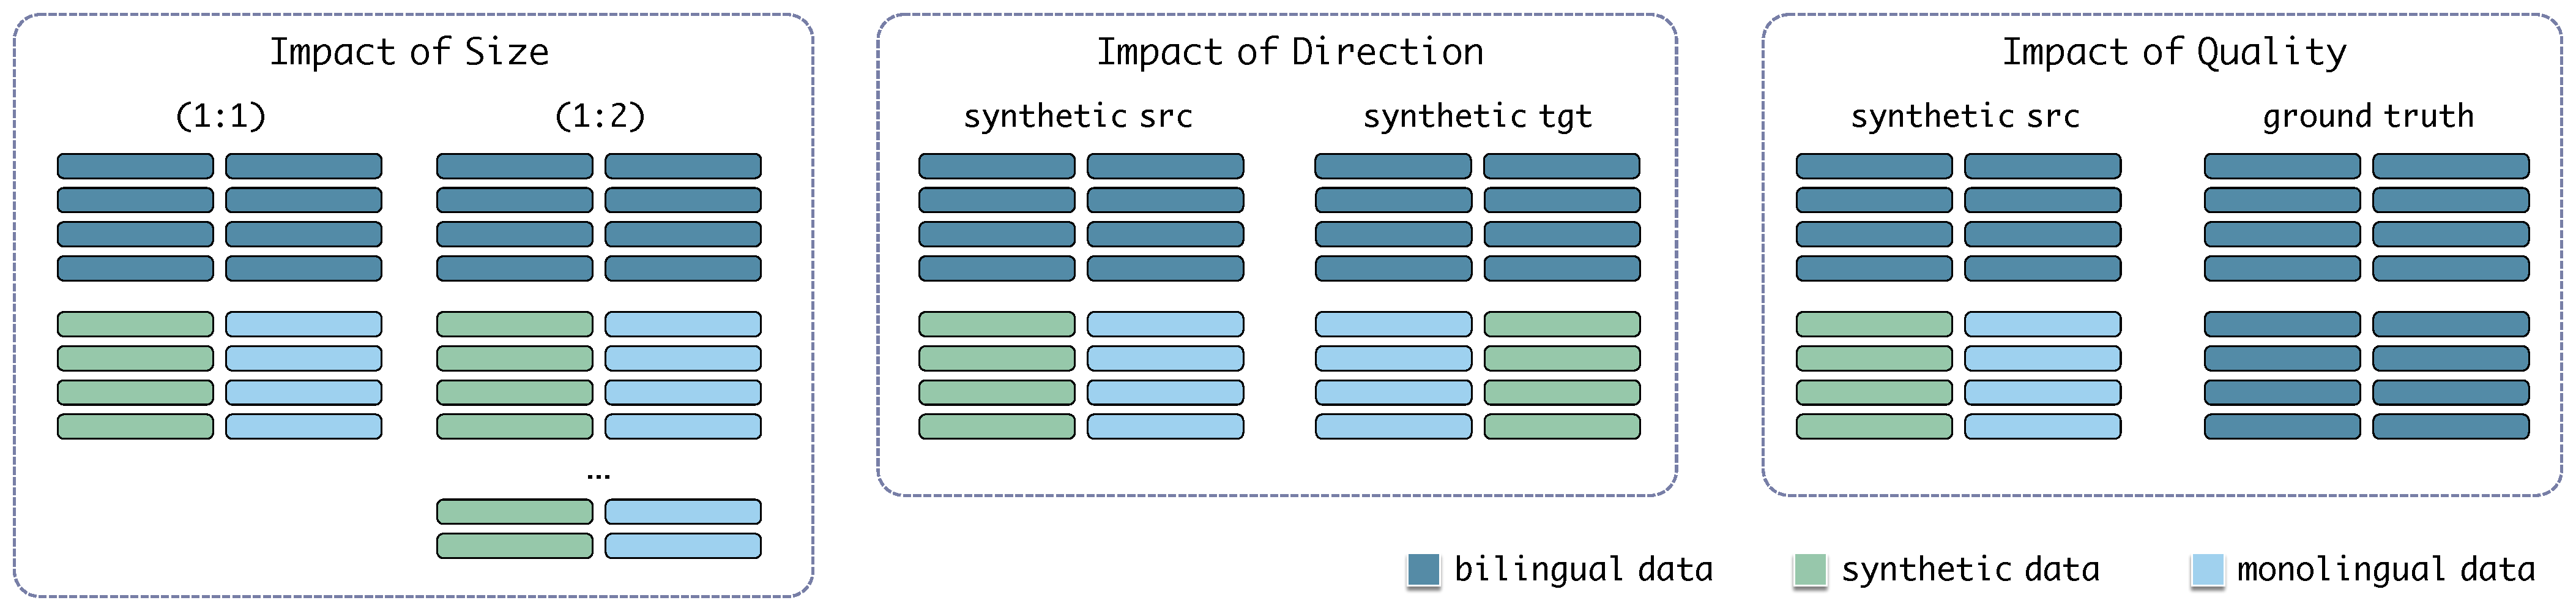
\includegraphics[width=\textwidth]{05-research-03/figs/bttypes.pdf}
\caption{Illustration of three set of experiments analyzing different impacts of synthetic data as additional training data: \textit{size} (left), \textit{direction} (middle), and \textit{quality} (right). %Green indicates synthetic data and blue indicates real data generated manually.
}
\label{btmets}
\end{center}
\end{figure}


\section{Analyzing back-translation with random sampling} \label{btbtanalysis}

In this section, we investigate different aspects and modeling challenges of integrating the back-translation method into the NMT pipeline.
We are interested in investigating the impact of synthetic data on translation quality with random sampling augmentation (see Figure~\ref{btmets}).

\subsection{Impact of synthetic data size}

One selection criterion for using back-translation is the ratio of real to synthetic data.
\citet{sennrich-haddow-birch:2016:P16-11} showed that higher ratios of synthetic data lead to decreases in translation performance. 
%
In order to investigate whether improvements in translation quality increase with higher ratios of synthetic data, we perform three experiments with different sizes of synthetic data (see Figure~\ref{btmets}: left).
Figure~\ref{ppl} shows the perplexity as a function of training time for different sizes of synthetic data.

\begin{figure}[htb!]
\begin{center}
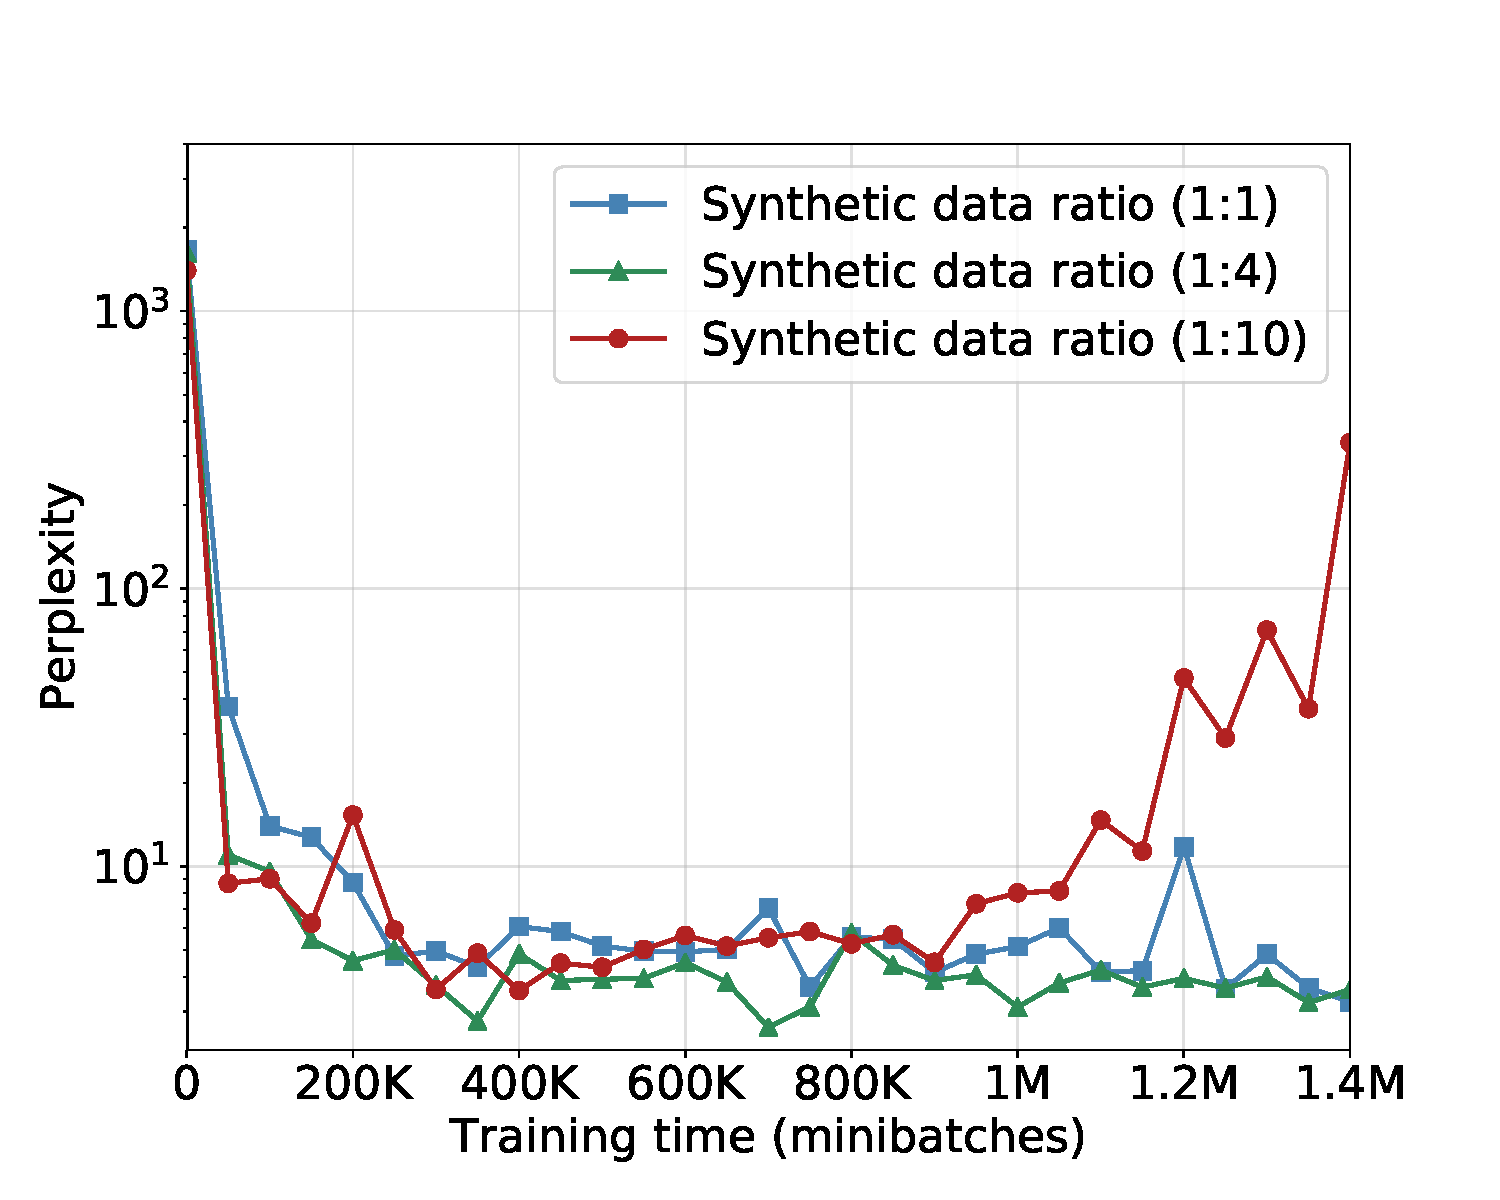
\includegraphics[width=0.8\textwidth]{05-research-03/figs/newppl}
\caption{Training plots for systems with different ratios of  (\mbox{$real:syn$}) training data, showing perplexity on development set.}
\label{ppl}
\end{center}
\end{figure}

We find that all systems perform similarly in the beginning and converge after observing increasingly more training instances.
However, the model with the ratio of (\mbox{1:10}) synthetic data becomes increasingly biased towards the noisy data after 1M instances.
Decreases in performance with more synthetic than real data is also in line with findings of \citet{2018arXiv180406189P}.
%
Comparing the systems using ratios of \mbox{1:1} and \mbox{1:4}, we see that the latter achieves lower perplexity during training.
Table~\ref{bigbigger} shows the performance of these systems on the German$\rightarrow$English translation task. 
%
\setlength{\tabcolsep}{4pt}
\begin{table}[htb!]
\begin{center}
\caption{\label{bigbigger} German$\rightarrow$English translation quality ({BLEU}) of systems with different ratios of \textit{\mbox{real:syn}} data.}
\begin{tabular}{lccccc}
 \toprule \bf  & \bf 	Size &  \bf WMT14 &  \bf	WMT15 &  \bf	WMT16 &  \bf	WMT17 \\ \midrule%
 Baseline	& 4.5M	& 26.7	&27.6	&32.5	&28.1\\
%Parallel + synthetic src (random)	& 8.9M	&	28.8	&30.0	&36.5	&31.1\\
%Parallel + synthetic src (random 2)	& 9M	& 28.9	&29.6&	36.2&	30.7\\
%Parallel + synthetic src (random 3)	& 9M	&	28.5	&29.6	&36.2&	30.6\\
\hspace{.15cm} + synthetic (\mbox{1:1})	& 9M	&	28.7&	29.7	&36.3	&30.8\\
\hspace{.15cm} + synthetic (\mbox{1:4}) 	&23M	&	29.1&	30.0&	36.9	&31.1\\
\hspace{.15cm} + synthetic (\mbox{1:10})  & 50M	&22.8&23.6&	29.2	&		 23.9\\
\bottomrule
\end{tabular}
\end{center}
\end{table}
%
The {BLEU} scores show that the translation quality does not improve linearly with the size of the synthetic data.
The model trained on \mbox{1:4} real to synthetic ratio of training data achieves the best results, however, the performance is close to the model trained on a ratio of \mbox{1:1}.

Similar to the study in this section, \citet{edunov-etal-2018-understanding} showed that it is possible to achieve the best results with a large-scale model trained on a \mbox{1:50} ratio of real to synthetic data. 
However, it is crucial to upsample the real data during training so that training batches contain on average an equal amount of real and synthetic data.




\subsection{Impact of translation direction}

Adding monolingual data in the target language to the training data has the potential benefit of introducing new contexts and improving the fluency of the translation model.
The automatically generated translations in the source language introduce new contexts for the source words and, despite not being perfect, improve the quality of the final re-trained model.

Monolingual data is available in large quantities for many languages. 
The decision of the direction of back-translation is subsequently not based on the monolingual data available, but on the advantage of having more fluent source or target sentences.

\begin{table}[htb!]
\begin{center}
\caption{\label{dir} English$\rightarrow$German translation quality ({BLEU}) of systems using forward and reverse models for generating synthetic data.}
\begin{tabular}{lccccc}
 \toprule \bf  & \bf 	Size &  \bf WMT14 &  \bf	WMT15 &  \bf	WMT16 &  \bf	WMT17 \\ \midrule%
Baseline	& 4.5M	&	21.2&	23.3&	28.0&	22.4\\
\hspace{.15cm} + synthetic tgt &	9M		&22.4	&25.3	&29.8	&23.7\\
\hspace{.15cm} + synthetic src &	9M		&24.0&	26.0	&30.7	&24.8\\
\bottomrule
\end{tabular}
\end{center}
\end{table}

\citet{Lambert:2011:ITM:2132960.2132997} showed that adding synthetic source and real target data achieves improvements in traditional phrase-based machine translation. Similarly, in previous works in NMT, back-translation is applied to monolingual data in the target language.
\citet{zhang-zong-2016-exploiting} proposed a self-learning algorithm to generate synthetic data from monolingual source sentences. 
During re-training, they distinguish between real and synthetic data by freezing the parameters of the decoder for the synthetic data.

We perform a small experiment to compare the impact of translation direction and where to incorporate monolingual data (see Figure~\ref{btmets}: middle).
Table~\ref{dir} shows that in both directions, the performance of the translation system improves over the baseline. 
%
This is in contrast to the findings of~\citet{Lambert:2011:ITM:2132960.2132997} for PBMT systems where they show that using synthetic target data does not lead to improvements in translation quality.

Still, when back-translating target monolingual data, BLEU scores in the target language are higher than when translating monolingual data in the source language. 
This indicates the importance of having fluent sentences in the target language.



\subsection{Impact of quality of the synthetic data}

One selection criterion for back-translation is the quality of the synthetic data.
\citet{W18-2709} studied the effects of noise in the training data on a translation model and discovered that NMT models are less robust to many types of noise than PBMT models.
In order for the NMT model to learn from the parallel data, the data should be fluent and close to the manually generated translations.
However, automatically generating sentences using back-translation is not as accurate as manual translations. 


To investigate the \textit{oracle gap} between the performance of manually created and back-translated sentences, we perform a simple experiment using the existing parallel training data (see Figure~\ref{btmets}: right).
In this experiment, we divide the parallel data into two parts, train the reverse model on the first half of the data, and use this model to back-translate the second half.
The manually translated sentences of the second half are considered as ground truth for the synthetic data.

Table~\ref{groundt} shows the {BLEU} scores of the experiments.
As to be expected, re-training with additional parallel data yields higher performance than re-training with additional synthetic data.
However, the differences between the {BLEU} scores of these two models are surprisingly small.
%
%
\begin{table}[htb!]
\begin{center}
\caption{\label{groundt} German$\rightarrow$English translation quality ({BLEU}) of systems using synthetic source and human generated source data.}
\begin{tabular}{lccccc}
 \toprule \bf  & \bf  Size  &  \bf WMT14 &  \bf	WMT15 &  \bf	WMT16 &  \bf	WMT17 \\ \midrule%
Baseline  &	2.25M	&24.3	&24.9	&29.5	&25.6\\
\hspace{.15cm} + synthetic src &	4.5M	 &26.0	&26.9	&32.2	&27.5\\
\hspace{.15cm} + ground truth	& 4.5M	& 26.7	&27.6	&32.5	&28.1\\
\bottomrule
\end{tabular}
\end{center}
\end{table}
%
This indicates that performing back-translation with a reasonably good reverse model already achieves results that are close to a system that uses additional manually translated data.
This is in line with findings of \citet{sennrich-haddow-birch:2016:P16-11} who observed that the same monolingual data translated with three translation systems of different quality and used in re-training the translation model yields similar results. 


\section{Back-Translation and token prediction loss} \label{bttokpred}

In the previous section, we observed that using back-translated data yields almost the same improvements as gold parallel data with the same target side.
However, there is a limit in learning from synthetic data, and with higher ratios of synthetic data the model biases too much towards the synthetic data.

In this section, we investigate the influence of the sampled sentences on the model.
In Chapter~\ref{chapter:research-02}, we showed that targeting specific words during data augmentation improves the generation of these words in the right context. 
Specifically, adding synthetic sentences containing those words to the training data has an impact on the prediction probabilities of individual words.
In this chapter, we further examine the effects of the back-translated synthetic data on the prediction of target tokens.

As mentioned in Section~\ref{nmtsec}, the objective function of training an NMT system is to minimize $\mathcal{L}$ by minimizing the prediction loss, $-\log p(y_t \mid \vt{y}_{<t}, \vt{s}_n)$, for each target token in the training data, where:
\begin{align}
p(y_t \mid y_{<t}, \vt{s}_n) =  \softmax \,(\vt{W}_o\widetilde{\vt{h}}_t)
\end{align}

\noindent Here, $\widetilde{\vt{h}}_t$ is the top hidden layer of the decoder and $\vt{W}_o$ is the output weight matrix. 
The addition of monolingual data in the target language improves the estimation of the probability $p({Y})$ and consequently, the model generates more fluent sentences.

\begin{figure}[htb!]
\centering
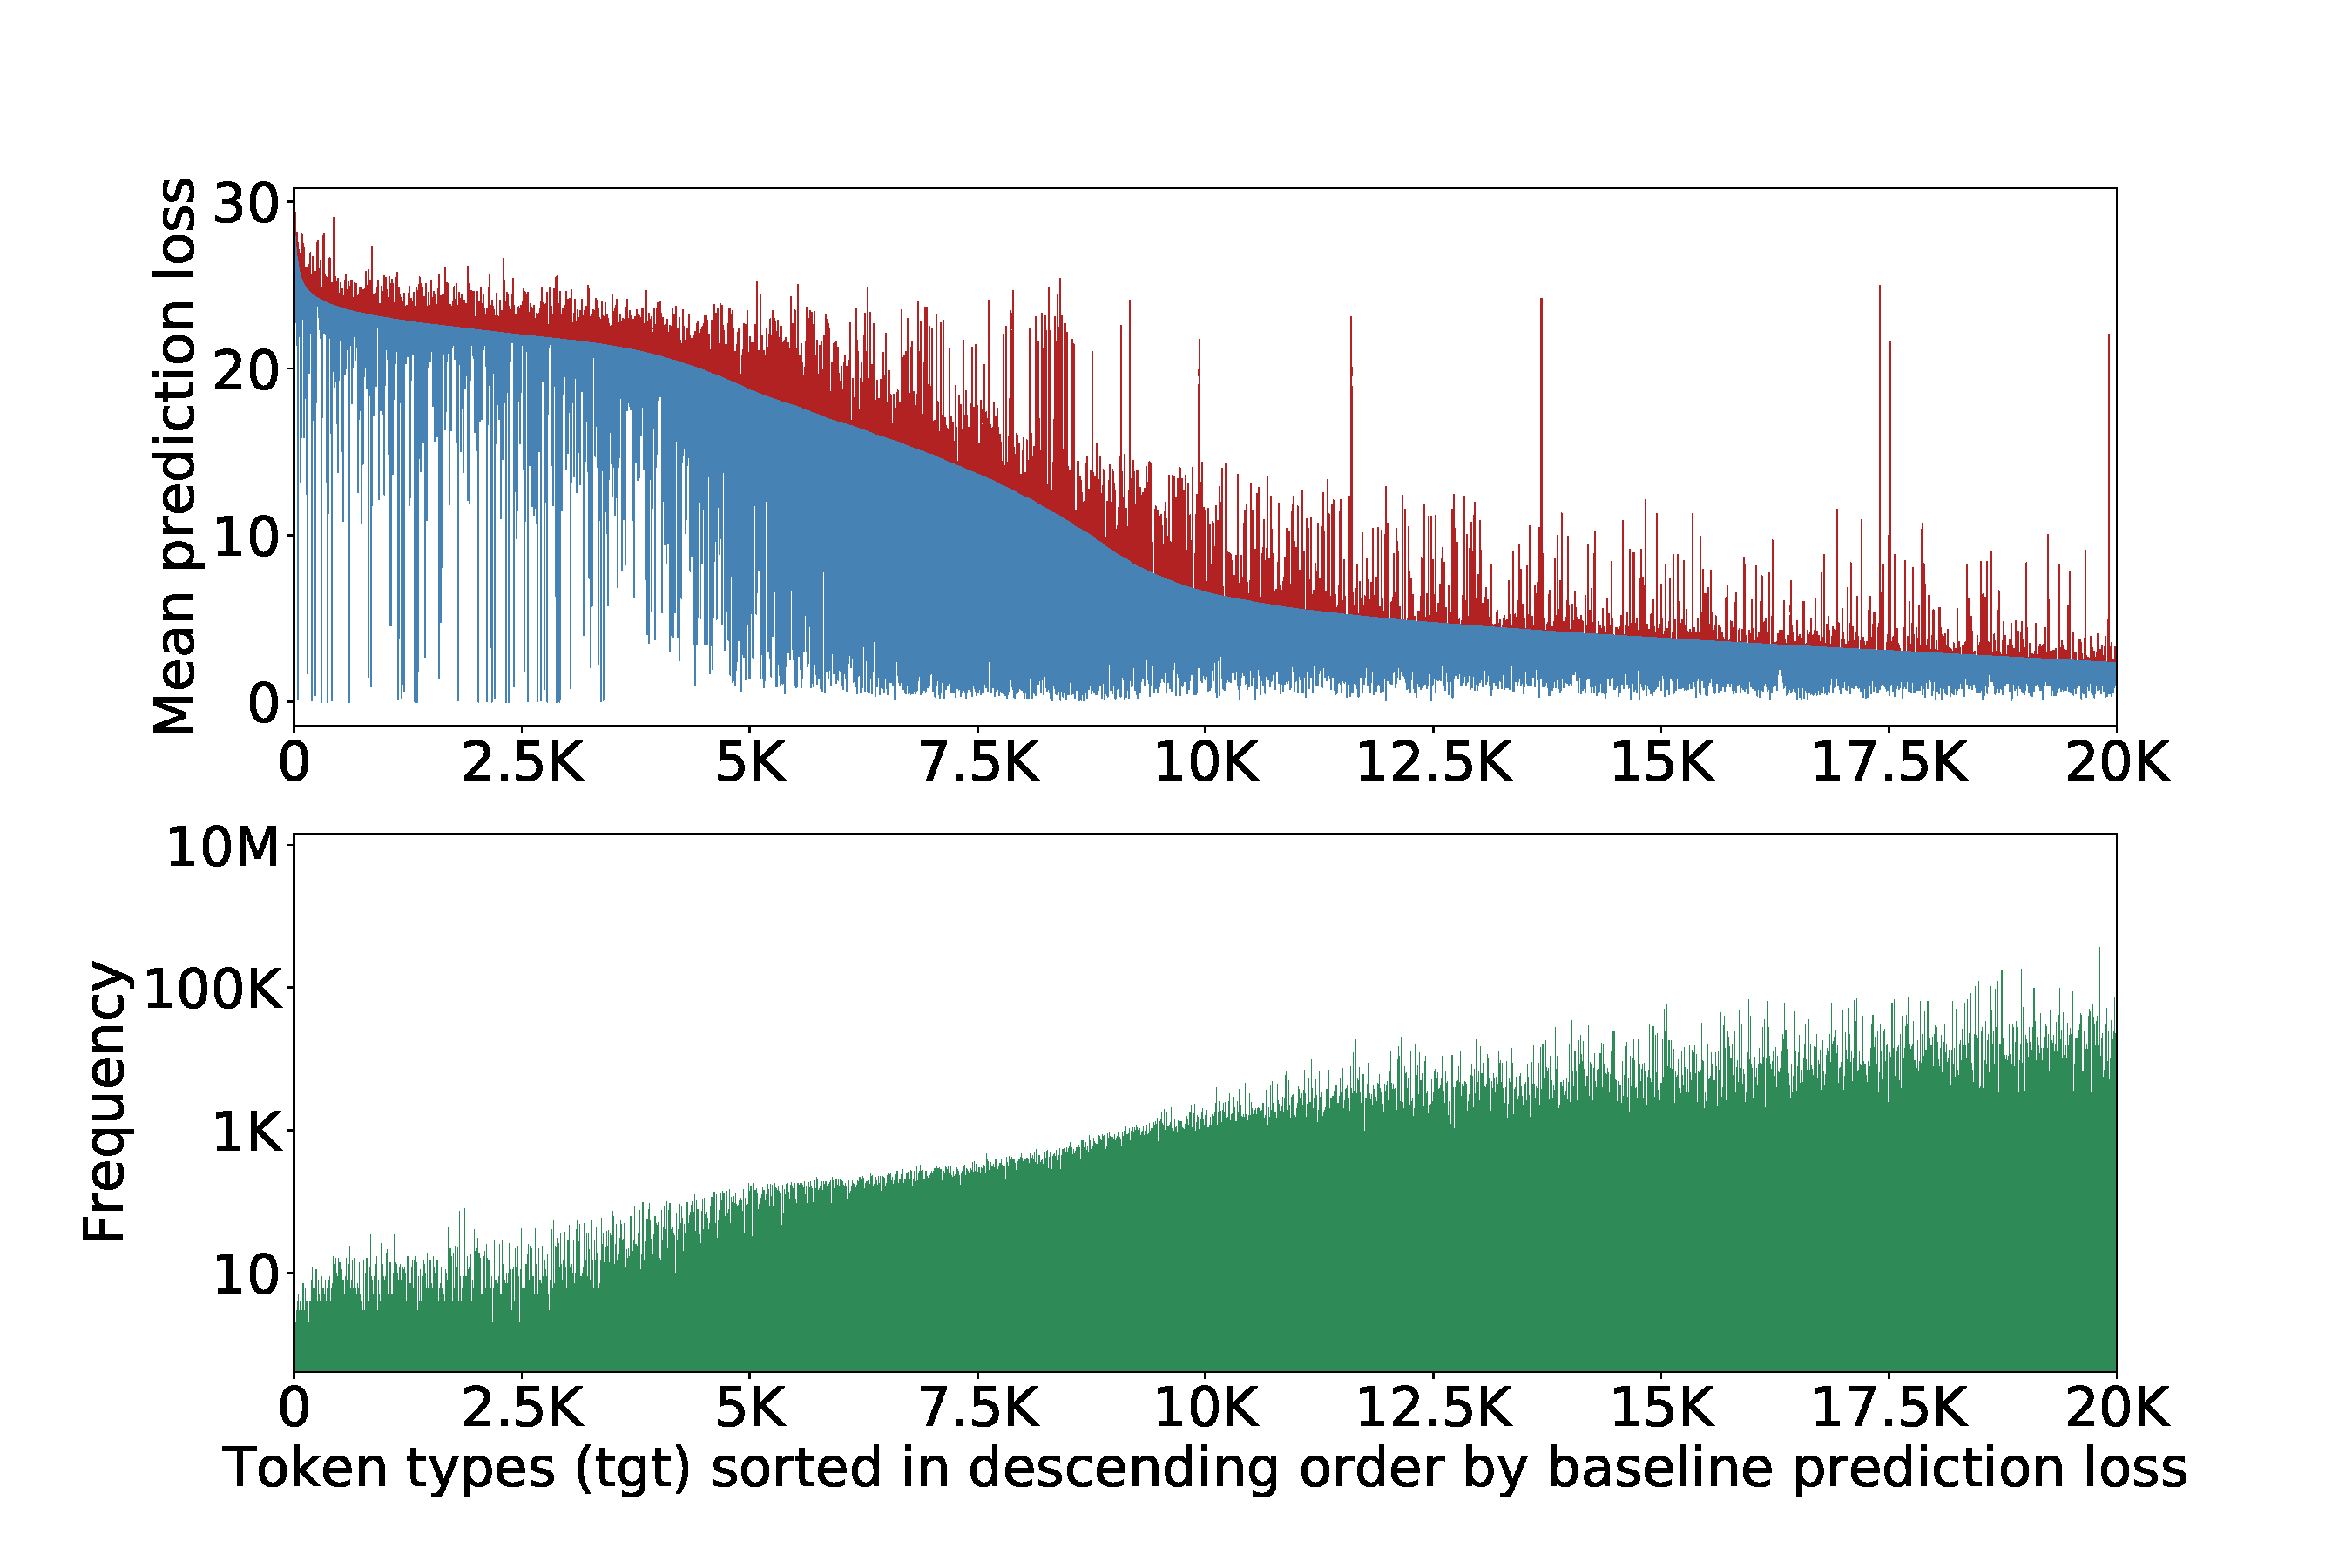
\includegraphics[width=\textwidth]{05-research-03/figs/newattemptoneall2}
\caption{Top: Changes in mean prediction loss after re-training with synthetic data sorted by mean prediction loss of the baseline system (x-axis). Decreases and increases in values are marked blue and red, respectively. Bottom: Frequencies (log) of target tokens in the baseline training data. Note that data points in both plots (x-axis) represent \textit{token} types in the vocabulary.}
\label{loss}
\end{figure}

\citet{sennrich-haddow-birch:2016:P16-11} show that by using back-translation, the system with target-side monolingual data reaches a lower perplexity on the development set.
This is expected since the domain of the monolingual data is news and therefore similar to the domain of the development set.
To investigate the model's accuracy independently from the domains of the data, we collect statistics of the target token prediction loss during training.

Figure~\ref{loss} shows the changes of token prediction loss % $-\log p(y_t | y_{<t}, \vt{s}_n)$ 
when training is close to converging and the weights are verging on being stable.
The values are sorted in decreasing order by the tokens' mean prediction losses of the system trained on real parallel data (before augmentation).
%
We observe an effect similar to distributional smoothing \citep{chen1996empirical}: 
First, we observe that the prediction loss increases slightly for most tokens (red).
Next, we spot an irregular pattern in \textit{decrease} of prediction loss (blue).
The largest decrease in loss occurs for tokens with high prediction loss values when trained on the parallel data only. 
This indicates that by randomly sampling sentences for back-translation, the model improves its estimation of tokens that were originally more difficult to predict, i.e., tokens that had a high prediction loss. 

Note that we compute the token prediction loss, without updating the weights, in just one pass over the training corpus with the final model and as a result, the loss is not biased towards the order of presentation of the training sentences.
% it is not biased towards the order of the data.

This finding motivates us to further explore sampling criteria for back-translation that contribute considerably to the parameter estimation of the translation model. 
We propose that by oversampling sentences containing difficult-to-predict tokens, we can maximize the impact of using the monolingual data.
After translating sentences containing such tokens and including them in the training data, the model becomes more robust in predicting these tokens.
In the next two sections, we propose several methods of using the target token prediction loss to identify the most beneficial sentences for back-translation and re-training the translation model. 


\section{Targeted sampling based on model failure} \label{bttarget}

One of the main benefits of using synthetic data is getting a better estimation of words that were originally difficult to predict as measured by their high prediction losses during training.
In this section, we propose four variations of how to identify these words and perform sampling to target these words.
The first three variations are described in Algorithm~\ref{alg1} where the list of difficult tokens is defined in two different ways.
The third variation is described in Algorithm~\ref{alg2}. 
The following subsections provide details of these model variants. 

 {\centering
\begin{minipage}{.85\linewidth}
\begin{algorithm}[H]
\caption{Sampling for difficult words}\label{alg1}
 \hspace*{\algorithmicindent} {\textbf{Input:}} Difficult tokens \textit{$\mathfrak{D}=\{y_i\}_{i=1}^{D}$}, monolingual 
corpus \textit{$\mathbb{M}$}, number \\
\hspace*{\algorithmicindent} of required samples \textit{N}   \\
\hspace*{\algorithmicindent} {\textbf{Output:}} Sampled sentences $S=\{S_i\}_{i=1}^{N}$ where each
sentence $S_i$ is \\
\hspace*{\algorithmicindent} sampled from $\mathbb{M}$
 \begin{algorithmic}[1]
\Procedure{\textsc{DiffSampling} ($\mathfrak{D}, \mathbb{M}, N$):}{}
%\State Initialize $D = \{\}$ \Comment{list of difficult words}
\State Initialize $S=\{\}$ %\Comment{sampled sentences set}
\Repeat
\State Sample $S_c$ from $\mathbb{M}$
\ForAll{tokens $y$ in $S_c$}
\If{$y \in \mathfrak{D}$} 
	\State Add $S_c$ to $S$
\EndFor
\Until{$|S| = N$}
\State \textbf{return} $S$ %\Comment{The gcd is b}
\EndProcedure
\end{algorithmic}
\end{algorithm}
\end{minipage}
\par
}
\vspace{\baselineskip}% Insert a blank line


\subsection{Token frequency as a feature of difficulty} 

Figure~\ref{loss} shows that the majority of tokens with high mean prediction losses have low frequencies in the training data.
Additionally, the majority of decreases in prediction loss after adding synthetic sentence pairs to the training data occurs with less frequent tokens.
Note that these tokens are not necessarily \textit{rare} and some of them may have up to 1000 different occurrences in the training data.
We observe in Figure~\ref{loss} that approximately half of the tokens in the target vocabulary benefit from back-translated data.

We propose a sampling criterion based on token frequencies. 
Sampling new contexts from monolingual data provides context diversity proportional to the token frequencies and less frequent tokens benefit most from new contexts.
Algorithm~\ref{alg1} presents this approach where the list of difficult tokens is defined as: 
\begin{align}
\mathfrak{D} = \{\forall y_i \in V_t \colon freq(y_i) < \eta \}
\end{align}
\noindent where $V_t$ is the target vocabulary and $\eta$ is the frequency threshold for deciding on the difficulty of the token.

\subsection{Tokens with high mean prediction losses}

In this approach, we use the mean losses to identify difficult-to-predict tokens. 
The mean prediction loss $\hat{\ell}(y)$ of token $y$ during training is defined as follows:
\begin{align}\label{ave}
\hat{\ell}(y) = \frac{1}{n_y}\sum_{n=1}^{N}\sum_{t=1}^{|Y^{n}|} -\log p(y^{n}_t \mid {y}^{n}_{<t}, \vt{s}_n) \delta(y^n_t,y)
\end{align}
%
where $n_y$ is the number of times token $y$ is observed during training, i.e., the token frequency of $y$, $N$ is the
number of sentences in the training data, $|\vt{Y}^{n}|$ is the length of target sentence $n$, and $\delta(y^n_t,y)$ is the Kronecker delta function, which is 1 if $y^n_t = y$ and 0 otherwise.
By specifically providing more sentences for difficult words, we improve the model's estimation and decrease its prediction uncertainty.

%During sampling from the monolingual data, we select sentences that contain difficult words.

Algorithm~\ref{alg1} presents this approach where the list of difficult tokens is defined as: 
\begin{align}
\mathfrak{D} = \{\forall y_i \in V_t \colon \hat{\ell}(y_i) > \mu \}
\end{align}

\noindent
where $V_t$ is the vocabulary of the target language and $\mu$ is the threshold for the difficulty of the token.

\subsection{Tokens with skewed prediction losses}

By using the mean loss for target tokens as defined above, we do not discriminate between differences in prediction loss for occurrences in different contexts. This lack of discrimination can be problematic for tokens with high loss variations. For instance, there can be a token with ten occurrences, out of which two have high and eight have low prediction loss values. 

We hypothesize that if a particular token is easier to predict in some contexts and harder in others, the sampling strategy should be context-sensitive, allowing to target specific contexts in which a token has a high prediction loss. 
%
In order to distinguish between tokens with a skewed and tokens with a more uniform prediction loss distribution, we use both the mean and standard deviation of the token prediction losses to identify difficult tokens.
Hence, we target tokens that have both high mean prediction loss and high amount of variation in different contexts.
%
Algorithm~\ref{alg1} formalizes this approach where the list of the difficult tokens is defined as: 
\begin{align}
\mathfrak{D} = \{\forall y_i \in V_t \colon \hat{\ell}(y_i) > \mu \land \sigma(\ell(y_i)) > \rho \}
\end{align}

\noindent where $\hat{\ell}(y_i)$ is the mean and $\sigma(\ell(y_i))$ is the standard deviation of prediction loss of token $y_i$, $V_t$ is the vocabulary list of the target language, and $\mu$ and $\rho$ are the thresholds for deciding the difficulty of the token.


 \subsection{Preserving sampling ratio of difficult occurrences}

Above, we examined the mean of prediction loss for each token over all occurrences, in order to identify difficult-to-predict tokens.
However, the uncertainty of the model in predicting a difficult token varies for different occurrences of the token: one token can be easy to predict in one context, and hard in another.
While the sampling step in the previous approaches targets these tokens, it does not ensure that the distribution of sampled sentences is similar to the distribution of problematic tokens in difficult contexts.

{\centering
\begin{minipage}{.85\linewidth}
\begin{algorithm}[H]
\caption{Sampling with ratio preservation}\label{alg2}
 \hspace*{\algorithmicindent} \textbf{Input:} Difficult tokens and the corresponding sentences in the bitext \\
  \hspace*{\algorithmicindent}  \textit{$\mathfrak{D}=\{y_t, Y_{y_t}=[y_1, \ldots, y_t, \ldots, y_m]\}$}, monolingual corpus \textit{$\mathbb{M}$}, \\
  \hspace*{\algorithmicindent} number of required samples \textit{N} \\
\hspace*{\algorithmicindent} \textbf{Output:} Sampled sentences $S=\{S_i\}_{i=1}^{N}$ where each sentence $S_i$ is \\
\hspace*{\algorithmicindent}  sampled from $\mathbb{M}$
 \begin{algorithmic}[1]
\Procedure{\textsc{PredLossRatioSampling}($\mathfrak{D}, \mathbb{M}, N$): }{}
\State Initialize $S=\{\}$
\State $H(y_t) = \frac{ N \times \mid(y_t, \boldsymbol{\cdot})\in \mathfrak{D}\mid}{\mid(y_{\boldsymbol{\cdot}}, \boldsymbol{\cdot})\in \mathfrak{D}\mid}$
%\State Initialize $H = []$ \Comment{Hash of difficult words and intended ratio in the sampled set}
\Repeat
\State Sample $S_c$ from $\mathbb{M}$
\ForAll{tokens $y$ in $S_c$}
\If{$|y \in S| < H(y)$} 
	\State Add $S_c$ to $S$
\EndFor
\Until{$|S| = N$}
\State \textbf{return} $S$ %\Comment{The gcd is b}
\EndProcedure
\end{algorithmic}
\end{algorithm}
\end{minipage}
\par
}
\vspace{\baselineskip}% Insert a blank line


To address this issue, we propose an approach where we consider the number of times a token occurs in difficult-to-predict contexts and sample sentences accordingly, thereby ensuring the same ratio as the distribution of difficult contexts.
If token $y_1$ is difficult to predict in two contexts and token $y_2$ is difficult to predict in four contexts, the number of sampled sentences containing $y_2$ is double the number of sampled sentences containing $y_1$.
Algorithm~\ref{alg2} formalizes this approach.
 


 \subsection{Results}
 
We measure the translation quality of various models for German$\rightarrow$English and English $\rightarrow$ German translation tasks.
As baseline we compare our approach to \citet{sennrich-haddow-birch:2016:P16-11}. 
For all experiments we sample and back-translate sentences from WMT monolingual data, keeping a one-to-one ratio of back-translated versus original data (\mbox{1:1}).
We set the hyperparameters $\mu$, $\rho$, and $\eta$ to 5, 10, and 5000, respectively.
The values of the hyperparameters are chosen on a small sample of the parallel data based on the token loss distribution. 

\begin{figure}[htb!]
\begin{center}
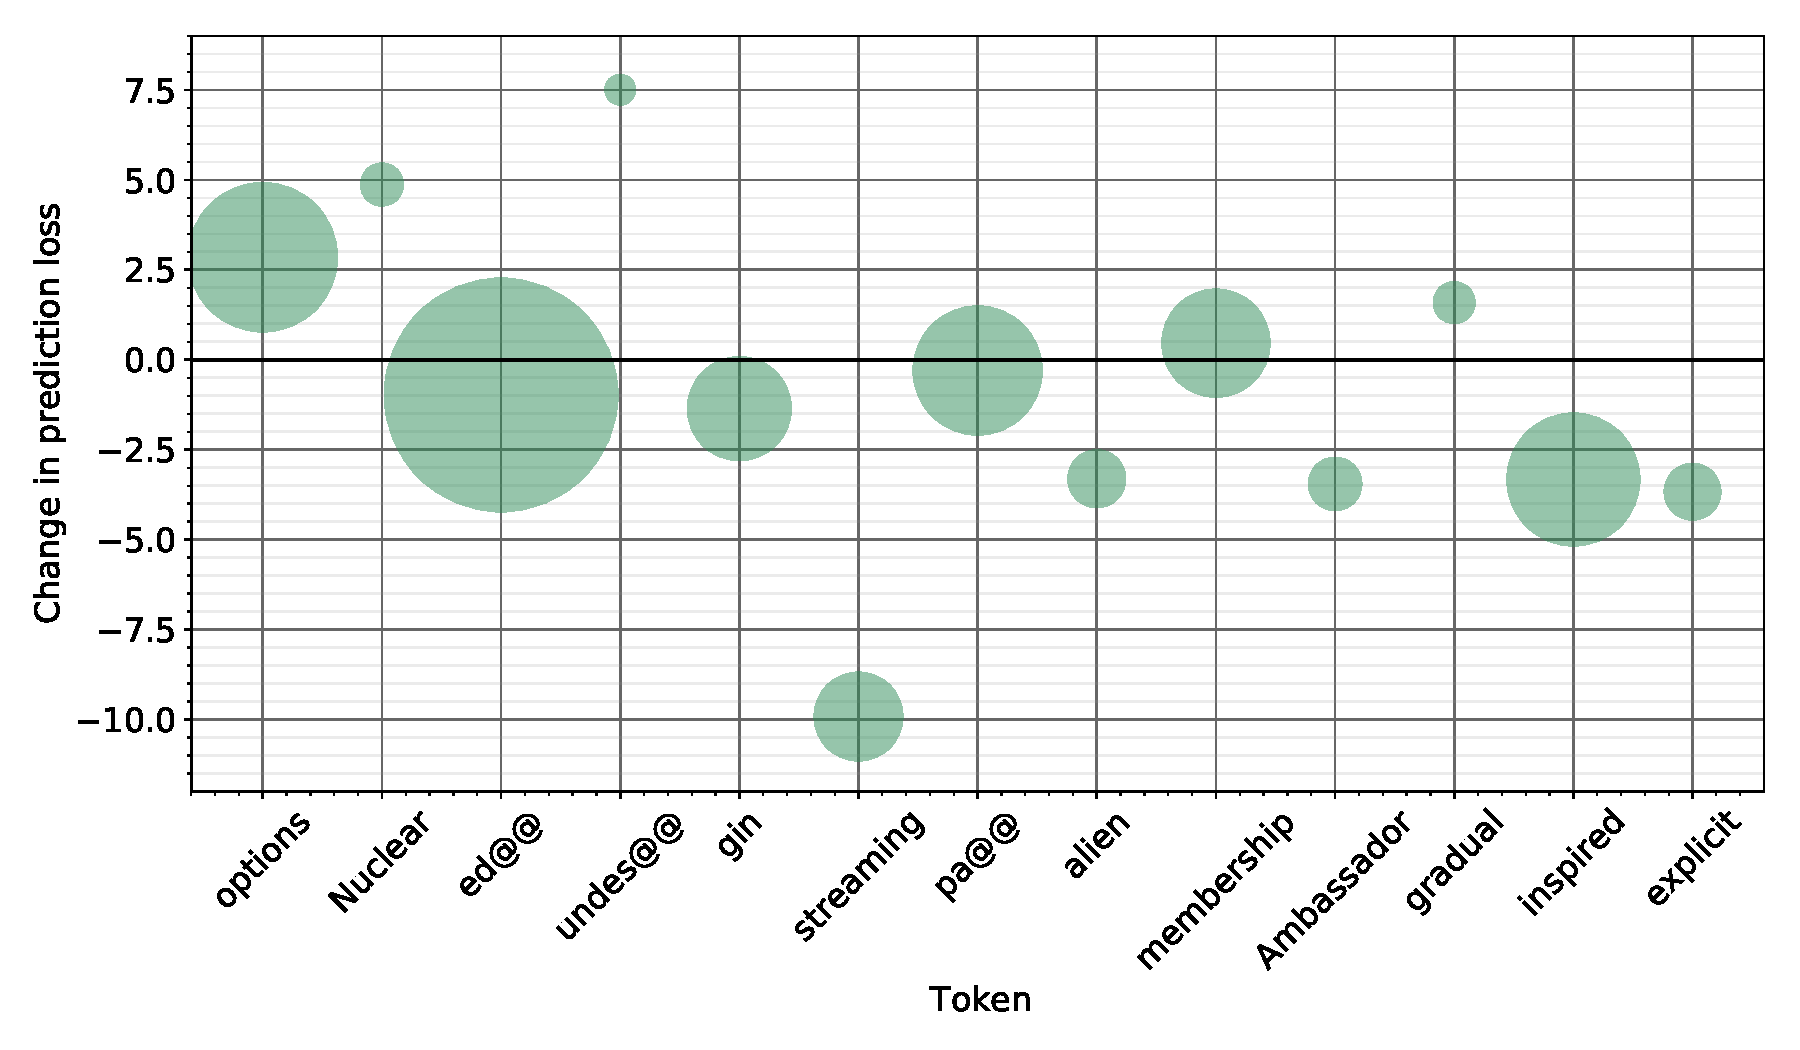
\includegraphics[width=\textwidth]{05-research-03/figs/changeinloss}
\caption{Examples of changes in average prediction loss after augmentation. Lower is better. The sizes of dots are proportional to the increase in the number of contexts for each word in the training data. Subword unit boundaries are marked with `@@'. \label{predlossexample}}
\end{center}
\end{figure}

Our proposed augmentation method increases instances of targeted words in the training data which leads to an overall decrease in average prediction loss per token. Figure~\ref{predlossexample} provides examples of tokens in the training data and their changes after data augmentation.  
The results of the translation experiments are presented in Tables~\ref{meanresultsende} and \ref{meanresultsdeen}.

\begin{table*}
\begin{center}
%\small%
\tabcolsep=2.5pt%
\caption{\label{meanresultsende}  English$\rightarrow$German translation quality ({BLEU}). Experiments marked $^\dagger$ are averaged over 3 runs. \textsc{Random} is the standard back-translation approach with random sampling. \textsc{MPL} and \textsc{Freq} are difficulty criteria based on mean prediction loss and token frequency, respectively. \textsc{MPL + sPL} is experiments with upsampling tokens with skewed prediction losses. \textsc{PPLR} preserves the  ratio of the distribution of difficult contexts.	}
\begin{tabular}{@{ }lccccc@{}}
\toprule
   & \multicolumn{4}{c}{\textbf{En-De}}  \\ \cmidrule{2-6} 
 \textbf{System}    &  \bf WMT14 &  \bf WMT15 &  \bf WMT16 &  \bf WMT17 \\ 
\midrule     
 \textsc{Baseline}$^\dagger$		& 21.2	&23.3&	28.0&	22.4\\
%Parallel + synthetic src (random)	& 8.9M	&	28.8	&30.0	&36.5	&31.1\\
%Parallel + synthetic src (random 2)	& 9M	& 28.9	&29.6&	36.2&	30.7\\
%Parallel + synthetic src (random 3)	& 9M	&	28.5	&29.6	&36.2&	30.6\\
\textsc{Random}$^\dagger$  &	 24.0&	26.0&	30.7	&24.8\\ \midrule
 \textbf{Difficulty criterion} & &&      \\ \midrule
%\textsc{PredLoss}, $n>=3$	& 	28.6	&	&29.3	&&	35.9	&&30.5&	&&&& &\\
\textsc{Freq} 	&24.2&27.0&31.7 &25.2\\			
\textsc{MPL}$^\dagger$	 &\textbf{24.7}&26.8&31.5&\textbf{25.5}\\ %$n>=1$	
\textsc{MPL + sPL} 	&24.1&26.9  &31.0&25.3\\
\textsc{PPLR}  &24.5&\textbf{27.2}&\textbf{31.8} &25.5\\
\bottomrule
\end{tabular}
\end{center}
\end{table*}

\begin{table*}
\begin{center}
\tabcolsep=2.5pt%
\caption{ \label{meanresultsdeen}  German$\rightarrow$English translation quality ({BLEU}). Experiments marked $^\dagger$ are averaged over 3 runs. \textsc{Random} is the standard back-translation approach with random sampling. \textsc{MPL} and \textsc{Freq} are difficulty criteria based on mean prediction loss and token frequency, respectively. \textsc{MPL + sPL} is experiments with upsampling tokens with skewed prediction losses. \textsc{PPLR} preserves the  ratio of the distribution of difficult contexts.	}
%\vspace{10mm}
\begin{tabular}{@{ }lccccc@{}}
\toprule
   & \multicolumn{4}{c}{\textbf{De-En}}  \\ \cmidrule{2-6}
 \textbf{System}  & \bf WMT14 & \bf  WMT15 &   \bf WMT16 &   \bf WMT17 \\ 
\midrule     
 \textsc{Baseline}$^\dagger$		& 26.7 &	27.6 &	32.5& 	28.1\\
%Parallel + synthetic src (random)	& 8.9M	&	28.8	&30.0	&36.5	&31.1\\
%Parallel + synthetic src (random 2)	& 9M	& 28.9	&29.6&	36.2&	30.7\\
%Parallel + synthetic src (random 3)	& 9M	&	28.5	&29.6	&36.2&	30.6\\
\textsc{Random}$^\dagger$ & 	28.7& 		29.7	&	36.3		&30.8 \\ \midrule
 \textbf{Difficulty criterion} & &&      \\ \midrule
%\textsc{PredLoss}, $>=3$	& 	28.6	&	&29.3	&&	35.9	&&30.5&	&&&& &\\
\textsc{Freq} 	& 29.7&30.5	&37.5&31.4 &\\		 	
\textsc{MPL}$^\dagger$ &	29.9 &		\textbf{30.9} 		&\textbf{37.8}	&\textbf{32.1}	\\ %$n>=1$	
%\textsc{MPL}, $\nless 3$ & 	28.6	&	29.3	&	35.9	&30.5 \\
\textsc{MPL + sPL} 	& 	\textbf{30.0}&		30.9		&37.7	&31.9  \\
\textsc{PPLR}	&		29.8	&30.9&37.4& 31.6  \\
\bottomrule
\end{tabular}
\end{center}
\end{table*}

As expected using random sampling for back-translation improves the translation quality over the baseline.
However, each of the proposed targeted sampling techniques outperforms random sampling. 
Specifically, the best performing model for German$\rightarrow$English uses the mean of prediction loss (\textsc{MPL}) for the target vocabulary to frequently sample sentences including these tokens.

For the English$\rightarrow$German experiments we obtain the best translation performance when we preserve the prediction loss ratio during sampling.
We also observe that even though the model targeting tokens with skewed prediction loss distributions ($\textsc{MPL + sPL}$) improves over random selection of sentences, it does not outperform the model using only mean prediction losses. 
Note that frequency-based sampling, the simplest method proposed in this chapter, is very effective.
We observe that the gains of other proposed approaches over frequency-based sampling are quite small. 
Therefore using frequency-based sampling remains a good strategy to improve translation quality over random sampling. 

\section{Context-Aware targeted sampling} \label{btcontextu}

In the previous section, we proposed methods for identifying difficult-to-predict tokens and performed targeted sampling from monolingual data.
While the objective was to increase the occurrences of difficult tokens, we ignored the context of these tokens in the sampled sentences. 

Arguably, if a word is difficult to predict in a given context, providing more examples of the same or similar context can aid the learning process.
In this section, we focus on the context of difficult-to-predict words and aim to sample sentences that are similar to the corresponding difficult context.
We first identify difficult-to-predict words and the local \textit{context} where the prediction loss is high. 
Next, we sample sentences from the monolingual data that contain a difficult-to-predict word. 
We then compare the context of the difficult word in the sampled sentence and the initial difficult context and select the sampled sentence if the contexts are similar. 
Finally, we back-translate the selected sentences and augment the training data.

{\centering
\begin{minipage}{.85\linewidth}
\begin{algorithm}[H]
\caption{Sampling with context}\label{alg3}
  \hspace*{\algorithmicindent} \textbf{Input:} Difficult tokens and the corresponding sentences  in the bitext \\
    \hspace*{\algorithmicindent}  \textit{$\mathfrak{D}=\{y_t, Y_{y_t}=[y_1, \ldots, y_t, \ldots, y_m]\}$},  monolingual corpus \textit{$\mathbb{M}$},  \\
      \hspace*{\algorithmicindent} context function \textit{$context$}, number of required samples \textit{N}, similarity \\
     \hspace*{\algorithmicindent} threshold $s$ \\
\hspace*{\algorithmicindent} \textbf{Output:} Sampled sentences $S=\{S_i\}_{i=1}^{N}$ where each sentence $S_i$ is \\
  \hspace*{\algorithmicindent} sampled from $\mathbb{M}$
 \begin{algorithmic}[1]
\Procedure{\textsc{contextSampling}($\mathfrak{D}, \mathbb{M}, context, N, s$): }{}
\State Initialize $S=\{\}$
\Repeat
\State Sample $S_c$ from $\mathbb{M}$
\ForAll{tokens $y_t$ in $S_c$}
	\If{$y_t \in \mathfrak{D}$} 
%\State $C_m \leftarrow substr(S_c,i-w, i+w)$
	\State $C_m \leftarrow context(S_c,$ index\_of$(S_c, y_t))$ \label{cont1}
	\ForAll{$Y_{y_t}$}
	%\State $C_p \leftarrow substr(Y_{y_t}, t-w, t+w)$
		\State $C_p \leftarrow context(Y_{y_t},$  index\_of$(Y_{y_t}, y_t)) $ \label{cont2}
                         \State \If{Sim$(C_m, C_p) > s$}  \label{simss}:  Add $S_c$ to $S$
	\EndFor
\EndFor
\Until{$|S| = N$}
\State \textbf{return} $S$ %\Comment{The gcd is b}
\EndProcedure
\end{algorithmic}
\end{algorithm}
\end{minipage}
\par
}
\vspace{\baselineskip}% Insert a blank line


The general algorithm is described in Algorithm~\ref{alg3}.
In the following sections, we discuss different definitions of the local context ($context$ function in line~\ref{cont1} and line~\ref{cont2}) and similarity measures ($\text{Sim}$ function in line~\ref{simss}) in this algorithm and report the results.

\subsection{Definition of local context}

Prediction loss is a function of the source sentence and the target context.
We hypothesize that one of the reasons that a token has a high prediction loss in only some contexts is because of the complexity of those contexts.
This complexity can be caused by an infrequent event such as a rare sense of the word, a domain that is different from other occurrences of the word, or an idiomatic expression. 

We identify \textit{pairs} of tokens and sentences from parallel data where in each pair, the NMT model suffers a high prediction loss for the token in the given context. 
Note that a token can occur several times in this list since it can be considered as difficult-to-predict in different sentences.

We propose two approaches to define the local context of a difficult token:

\paragraph{Neighboring tokens}

A straightforward way is to use positional context: tokens that precede and follow the target token, typically in a window of $w$ tokens to each side.
For sentence $S$ containing a difficult token at index $i$, the \textit{context} function in Algorithm~\ref{alg3} is:
\begin{align}
context(S, i) = [S^{i-w}, \ldots, S^{i-1}, S^{i+1}, \ldots, S^{i+w}]
\end{align}
\noindent
where $S^{j}$ is the token at index $j$ in sentence $S$.
Note that in this approach, we look at a window of fixed size and as a result, not all subwords from the same word may end up in this context window. For instance for the sentence \textit{`a professor and a \underline{colleague} at Stan$\mid$ford'}, with target word \textit{`colleague'}, and $w=2$, the context is [\textit{`and', `a', `at', `Stan'}]. Here, the subword \textit{`ford'} as part of the word \textit{`Stanford'} is not included in the context window. The symbol `$\mid$' signifies subword unit boundary. 

\paragraph{Sibling tokens}

In our analysis of prediction loss during training, we observe that several tokens that are difficult to predict are indeed subword units.
Current state-of-the-art NMT systems apply BPE to the training data to address large vocabulary challenges \citep{sennrich-haddow-birch:2016:P16-12}.
%
%
%
By using BPE, the model generalizes common subword units towards what is more frequent in the training data.
This is inherently useful since it allows for better learning of less frequent words.
However, a side effect of this approach is that at times the model generates subword units that are not linked to any words in the source sentence.
As an example, in Table~\ref{exbpe1}, the German source and the English reference translation highlight this problem.
The word \textit{`B$\mid$ahr'} consisting of two subword units is incorrectly translated into \textit{`B$\mid$risk'} because of an unintended side-effect of both sharing the subword unit \textit{`B'}.

We address the insufficiency of the context for subword units with high prediction losses by targeting these tokens in sentence sampling.
Algorithm~\ref{alg3} formalizes this approach in sampling sentences from the monolingual data.
For a sentence $S$ containing a difficult subword at index $i$, the context function is defined as:
\begin{align}
context(S, i) = [ S^{n},\ldots, S^{i-1}, S^{i+1}, \ldots, S^{m} ]
\end{align}
where every token $S^{j}$ in the local context is a subword unit and part of the same word as $S^i$.
Table~\ref{exbpe2} presents examples of sampled sentences for the difficult subword unit \textit{`Stan'}.
In this case, the difficult context for this token is \textit{`Stan$\mid$ford'} and we use it for computation of similarity.
This suggests that the subword unit \textit{`Stan'} is difficult to predict when the context is for the word \textit{`Stan$\mid$ford'}.
This excludes other contexts where the subword unit \textit{`Stan'} is part of another word, such as \textit{`Stan$\mid$dard'}.
%
\begin{table}[thb!]
\begin{center}\small
\caption{\label{exbpe1} An example from the synthetic data where the word \textit{B$\mid$ahr} is incorrectly translated to \textit{B$\mid$risk}. Subword unit boundaries are marked with `$\mid$'.}
\begin{tabularx}{0.7\columnwidth}{lX}
\toprule
\textit{source} & wer glaube, dass das Ende, sobald sie in Deutschland ank$\mid${\"a}$\mid$men, ir$\mid$re, erz{\"a}hlt \textbf{B$\mid$ahr}. \\
\textit{reference } & if you think that this stops as soon as they arrive in Germany, you'd be wrong, says \textbf{B$\mid$ahr}.\\
\textit{NMT output} & who believe that the end, as soon as they go to Germany, tells \textbf{B$\mid$risk}.\\
\bottomrule
\end{tabularx}
\end{center}
\end{table}
%
\begin{table}[htb!]
\begin{center}\small
\caption{\label{exbpe2} Results of context-aware targeted sampling with sibling tokens for the difficult subword unit \textit{`Stan'}. In this example, the difficult context in which the subword \textit{`Stan'} has a high prediction loss is the complete word \textit{`Stanford'} and we sample sentences containing this word.}
\begin{tabularx}{0.8\columnwidth}{Xr}
\toprule
 \textit{Sentence from bitext containing difficult token \textbf{`Stan'}} & \\ \midrule
\multicolumn{2}{X}{He attended \textit{\textbf{Stan}$\mid$ford} University, where he double maj$\mid$ored in Spanish and History.}  \\  
  \midrule
  \textit{Sampled sentences from monolingual data} & \\% \textit{Similarity} \\ 
  \midrule
   %$-$ 
  \rowcolor{tablegray}  The group is headed by Aar$\mid$on K$\mid$ush$\mid$ner, a \textit{\textbf{Stan}$\mid$ford} University gradu$\mid$ate who formerly headed a gre$\mid$eting card company. & \\% 0.74 \\ %0.74 
   Ford just opened a new R\&D center near \textit{\textbf{Stan}$\mid$ford} University, a hot$\mid$bed of such technological research. & \\%0.73 \\%0.73
   \rowcolor{tablegray} Joe Grund$\mid$fest, a professor and a colleague at \textit{\textbf{Stan}$\mid$ford} Law School, outlines four reasons why the path to the IP$\mid$O has become so steep for asp$\mid$iring companies. & \\% 0.73 \\%0.73
\bottomrule
\end{tabularx}
\end{center}
\end{table}

\subsection{Similarity of the local contexts}

In context-aware targeted sampling, we compare the context of a sentence candidate and the difficult context in the parallel data and select the sentence if they are \textit{similar}.
In the following, we propose two approaches for measuring the similarities. 

\paragraph{Matching the local context (Exct)}

In this approach, we aim to sample sentences containing the difficult token matching the exact context to the problematic context.
By sampling sentences that match in a local window with the problematic context and differ in the rest of the sentence, we have more instances of the difficult token for training.
Algorithm~\ref{alg3} formalizes this approach where the similarity function is defined as:
\begin{align}
\text{Sim}(C_m, C_p) = \frac{1}{c} \sum_{i=1}^{c}\delta(C_m^i, C_p^i)
\end{align}

\noindent $C_m$ and $C_p$ are the contexts of the sentences from monolingual and parallel data, respectively, and $c$ is the number of tokens in the contexts. The $\delta$ function returns 1 when $C_m^i$ and $C_p^i$ are the same token, and 0 otherwise. 

\paragraph{Word representations (Sem)}

Another approach to sampling sentences that are similar to the problematic context is to weaken the matching assumption.
Allowing sentences that are similar in subject and not match the exact context words allows for lexical diversity in the training data.
We use embeddings obtained by training the Skipgram model \citep{mikolov2013efficient} on monolingual data to calculate the similarity of the two contexts.
For this approach we define the similarity function in Algorithm~\ref{alg3} as:
\begin{align}
\text{Sim}(C_m, C_p)  = \cos(\vt{v}(C_m), \vt{v}(C_p))
\end{align}
where $\vt{v}(C_m)$ and $\vt{v}(C_p)$ are the averaged embeddings of the tokens in the contexts.
%
Table~\ref{context} gives examples of sampled sentences for the difficult word \textit{Rock}.
In this example, the context where the word \textit{`Rock'} has high prediction loss is about the \textit{music genre} and not the most prominent sense of the word, \textit{stone}.
Sampling sentences that contain this word in this particular context provides an additional signal for the translation model to improve parameter estimation. 

\begin{table}[htb!]
\begin{center}\small
\caption{\label{context} Results of context-aware targeted sampling for the difficult token \textit{`Rock'} }
\begin{tabularx}{0.89\columnwidth}{Xcc}
\toprule
 \textit{Sentence from bitext containing difficult word} & & \\ \midrule
  Bud$\mid$dy Hol$\mid$ly was part of the first group induc$\mid$ted into the \textbf{Rock} and R$\mid$oll Hall of F$\mid$ame on its formation in 1986. &  \\  \midrule
  \textit{Sentences from monolingual data} & \textit{Similarity} & \textit{Sampled} \\ \midrule
  \rowcolor{tablegray} A 2008 \textbf{Rock} and R$\mid$oll Hall of F$\mid$ame induc$\mid$t$\mid$ee, Mad$\mid$onna is ran$\mid$ked by the Gu$\mid$inn$\mid$ess Book of World Rec$\mid$ords as the top-selling recording artist of all time. & 0.86 & \cmark \\% (\textit{Sim=0.86}) \\
   The winners were chosen by 500 voters, mostly musicians and other music industry veter$\mid$ans, who belong to the \textbf{Rock} and R$\mid$oll Hall of F$\mid$ame Foundation.  & 0.81 & \cmark \\
  \rowcolor{tablegray} The \textbf{Rock} and R$\mid$oll Hall of Fam$\mid$ers gave birth to the California rock sound. & 0.79& \cmark  \\%(\textit{Sim=0.79}) \\
 After an ice cold San Miguel beer at the H$\mid$ard \textbf{Rock} Caf\'e (Ay$\mid$ala Center) just enter the Bur$\mid$gos Street and enjoy the different clubs. & 0.42 & \xmark \\
  \rowcolor{tablegray}  See a play on Broad$\mid$way, enjoy stunning views from the Top of the \textbf{Rock}, or spend the day at the Museum of Mo$\mid$dern Art, all situated nearby. & 0.34 & \xmark  \\
The Library received the donations and endo$\mid$w$\mid$ments of prominent individuals such as John D. \textbf{Rock}$\mid$ef$\mid$eller and James B. Wil$\mid$b$\mid$ur. & 0.29 & \xmark  \\
\bottomrule
\end{tabularx}
\end{center}
\end{table}

 \subsection{Results}

\begin{table*}[p]
	\centering
	\setlength{\tabcolsep}{6pt}
\rotatebox{90}{
\begin{minipage}{\textheight}
\begin{center}
\caption{\label{contextresultsdeen} German$\rightarrow$English translation quality ({BLEU}). Experiments marked $^\dagger$ are averaged over 3 runs. \textsc{Random} is the standard back-translation approach with random sampling. \textsc{PredLoss} is the contextual prediction loss and \textsc{MPL} is the average loss. \textit{token} and \textit{SubUnit} are context selection definitions from neighboring tokens and subword units, respectively. Note that token includes both subword units and full words. \textit{Sent} regards the entire sentence as the context. \textit{Sem} is computing context similarities with token embeddings and \textit{Exct} is comparing the context tokens.}
\begin{tabular}{lcccccccccc}
\toprule
 &&&&&& \multicolumn{4}{c}{\textbf{De-En}}   \\  \cmidrule{7-11} 
 \textbf{System}   && &&&&  \bf WMT14 & \bf WMT15 & \bf WMT16 & \bf WMT17   \\ 
 \midrule    
 \textsc{Baseline} $^\dagger$ & &&&&& 26.7 &	27.6 &	32.5	&28.1\\
%Parallel + synthetic src (random)	& 8.9M	&	28.8	&30.0	&36.5	&31.1\\
%Parallel + synthetic src (random 2)	& 9M	& 28.9	&29.6&	36.2&	30.7\\
%Parallel + synthetic src (random 3)	& 9M	&	28.5	&29.6	&36.2&	30.6\\
\textsc{Random} $^\dagger$ & &&&&&  28.7& 		29.7	&	36.3	&	30.8\\ \midrule
\multirow{2}{*}{ \textbf{Difficulty criterion}} & \multicolumn{3}{c}{\textbf{Context}} &  \multicolumn{2}{c}{\textbf{Similarity}}       \\   \cmidrule(lr){2-4}   \cmidrule(lr){5-6}   %\midrule
   & Neighbor & Sibling& Sentence & Exct & Sem   &    \\ \midrule
\textsc{Freq} & \cmark && & & \cmark  &	 30.0&30.8&37.6&31.7  \\	
\textsc{PredLoss} & &\cmark&  & \cmark &	& 29.1&30.1&	36.9&31.0\\			
%\textsc{PredLoss} & \textsc{Swords}  & \textsc{emb }	&29.6 &30.5&37.5	&31.7&&24.4&\textbf{27.5} &29.8&23.7\\			
\textsc{PredLoss}  & \cmark && &\cmark& 	&	29.7 & 	30.6	&37.6&	31.8  \\ %trigram-bi-uni
\textsc{PredLoss}  & \cmark && && \cmark	 &29.9&30.8	&37.7&31.9  \\
\textsc{PredLoss} & &  &\cmark& & \cmark 	& 24.9&	25.5	&30.1&	26.2   \\	
%\textsc{PredLoss},	&&  {semantic } & 		30.0&	30.7&	37.7	&31.6\\
%\textsc{PredLoss},  .fixed ratio?	&&	 {semantic } & 	29.0&	30.2&	36.6&	31.1\\
%\textsc{PredLoss},   noStop $+$ src	&&	 {semantic } &	30.0	&30.8	&37.7&	31.7\\		
%\midrule	
\textsc{MPL } & \cmark &&  & &\cmark &   \textbf{30.2}	&\textbf{31.4}	&\textbf{37.9}	&\textbf{32.2}\\
\bottomrule
\end{tabular}
\end{center}
\end{minipage}
}
\end{table*}


\begin{table*} [p]
	\centering
		\setlength{\tabcolsep}{6pt}
\rotatebox{90}{
\begin{minipage}{\textheight}
\begin{center}
\caption{\label{contextresultsende} English$\rightarrow$German translation quality ({BLEU}). Experiments marked $^\dagger$ are averaged over 3 runs. \textsc{Random} is the standard back-translation approach with random sampling. \textsc{PredLoss} is the contextual prediction loss and \textsc{MPL} is the average loss. \textit{token} and \textit{SubUnit} are context selection definitions from neighboring tokens and subword units, respectively. Note that token includes both subword units and full words. \textit{Sent} denotes the sentence as the context. \textit{Sem} is computing context similarities with token embeddings and \textit{Exct} is comparing the context tokens.}
\begin{tabular}{lcccccccccc}
\toprule
 &&&&&& \multicolumn{4}{c}{\textbf{En-De}}   \\ \cmidrule{7-11} 
 \textbf{System}   && &&&&  \bf WMT14 & \bf WMT15 & \bf WMT16 & \bf WMT17   \\ 
 \midrule    
 \textsc{Baseline} $^\dagger$& &&&&&  21.2	&23.3&	28.0&	22.4\\
%Parallel + synthetic src (random)	& 8.9M	&	28.8	&30.0	&36.5	&31.1\\
%Parallel + synthetic src (random 2)	& 9M	& 28.9	&29.6&	36.2&	30.7\\
%Parallel + synthetic src (random 3)	& 9M	&	28.5	&29.6	&36.2&	30.6\\
\textsc{Random} $^\dagger$ & &&&&&	 24.0&	26.0&	30.7	&24.8\\ \midrule
\multirow{2}{*}{ \textbf{Difficulty criterion}} & \multicolumn{3}{c}{\textbf{Context}} &  \multicolumn{2}{c}{\textbf{Similarity}}       \\   \cmidrule(lr){2-4}   \cmidrule(lr){5-6}   %\midrule
   & Neighbor & Sibling& Sentence & Exct & Sem   &    \\ \midrule
\textsc{Freq} & \cmark && &  & \cmark  &	 24.4 &   26.3 &31.5&25.6 \\	
\textsc{PredLoss} & & \cmark & & \cmark &		&23.8&26.2 &28.8&23.2\\			
%\textsc{PredLoss} & \textsc{Swords}  & \textsc{emb }	&29.6 &30.5&37.5	&31.7&&24.4&\textbf{27.5} &29.8&23.7\\			
\textsc{PredLoss} & \cmark && & \cmark & 	&	 24.3  &27.4&31.6 & 25.5\\ %trigram-bi-uni
\textsc{PredLoss} &\cmark && & & \cmark & 24.5  &\textbf{27.5}&31.7 & 25.6\\
\textsc{PredLoss} &&& \cmark  & & \cmark		 &22.0&	24.6&	27.9	&22.5\\					
\textsc{MPL } & \cmark &&  & &\cmark  &  \textbf{24.4}& 27.2&\textbf{31.8}&\textbf{25.6}\\
\bottomrule
\end{tabular}
\end{center}
\end{minipage}
}
\end{table*}


The results of the translation experiments are given in Tables~\ref{contextresultsdeen} and \ref{contextresultsende} for German$\rightarrow$ English and English$\rightarrow$German, respectively.
In these experiments, we set the hyperparameters $s$ and $w$ to 0.75 and 4, respectively.
Comparing the experiments with different similarity measures, \textit{Exct} and \textit{Sem}, we observe that in all test sets we achieve the best results when using word embeddings.
This indicates that for targeted sampling it is more beneficial to have diversity in the context of difficult words as opposed to having the exact n-grams. 
When using embeddings as the similarity measure, it is worth noting that with a context of size 4 the model performs very well but fails when we increase the window size to include the whole sentence. 
The experiments focusing on tokens from the same words ({sibling} tokens) achieve improvements over the baselines, however, they perform slightly worse than the experiments using {neighboring} tokens as context.

The best BLEU scores are obtained with the mean of prediction loss as difficulty criterion (\textsc{MPL}) and using word representations to identify the most similar contexts.
We observe that summarizing the distribution of the prediction losses by its mean is more beneficial than using individual losses.
Our results motivate further explorations of using context for targeted sampling sentences for back-translation.


\section{Qualitative results} \label{btanalysisagain}

Finally, we review our proposed approach and further investigate individual token losses.
We observed that the \textit{individual} token loss, even after training converges, has a degree of instability and for the same word, it varies from context to context. 
However, in our experiments in the previous section, using local context to identify these difficult words was not very successful. 

We look at some examples from the training data where individual token loss is unstable in different contexts.
Figure~\ref{loosexamples} illustrates several sentences from the training data containing the subword \textit{`danger@@'} and the respective prediction losses of the trained model. The symbol `@@' signifies subword unit boundary. 
%
In all instances, this subword unit is part of the word \textit{`dangerously'}. 
All of the source sentences of these examples include the same German translation, \textit{`gef{\"a}hrlich'}, that corresponds to the translation of this word.
In this particular example, we see no clear indication in the context of why the model's confidence for the token \textit{`danger'} is considerably different for different contexts. 

\begin{figure}[htb!]
\begin{minipage}{\textwidth} 
\begin{center}

\includegraphics[width=\textwidth]{05-research-03/figs/sent1}    
\end{center}
\end{minipage}   
\par\smallskip % force a bit of vertical whitespace
\hspace{\fill}  %% no blank line before of after this instruction
%\begin{minipage}{\textwidth} 
%
\includegraphics[width=\textwidth]{05-research-03/figs/sent2}    %extra
%\end{minipage}    
%\hspace{\fill}  %% no blank line before of after this instruction
%\vspace{0.75cm}
\begin{minipage}{\textwidth} 

\includegraphics[width=\textwidth]{05-research-03/figs/sent3}    
\end{minipage}   
\par\smallskip % force a bit of vertical whitespace
\begin{minipage}{\textwidth} 

\includegraphics[width=\textwidth]{05-research-03/figs/sent4}    
\end{minipage}  
%\begin{minipage}{\textwidth} 
%
\includegraphics[width=\textwidth]{05-research-03/figs/sent5}     %extra
%\end{minipage}  
\caption{Visualization of token prediction loss (final training epoch) for the subword \textit{\textbf{danger@@}} in three different sentences. Darker means the model has less confidence predicting the word. Subword unit boundaries are marked with `@@' \label{loosexamples}}  
\end{figure}


Finally, we study the importance of the position of the token in the confidence of the model.
\begin{figure}[htb!]
\begin{center}
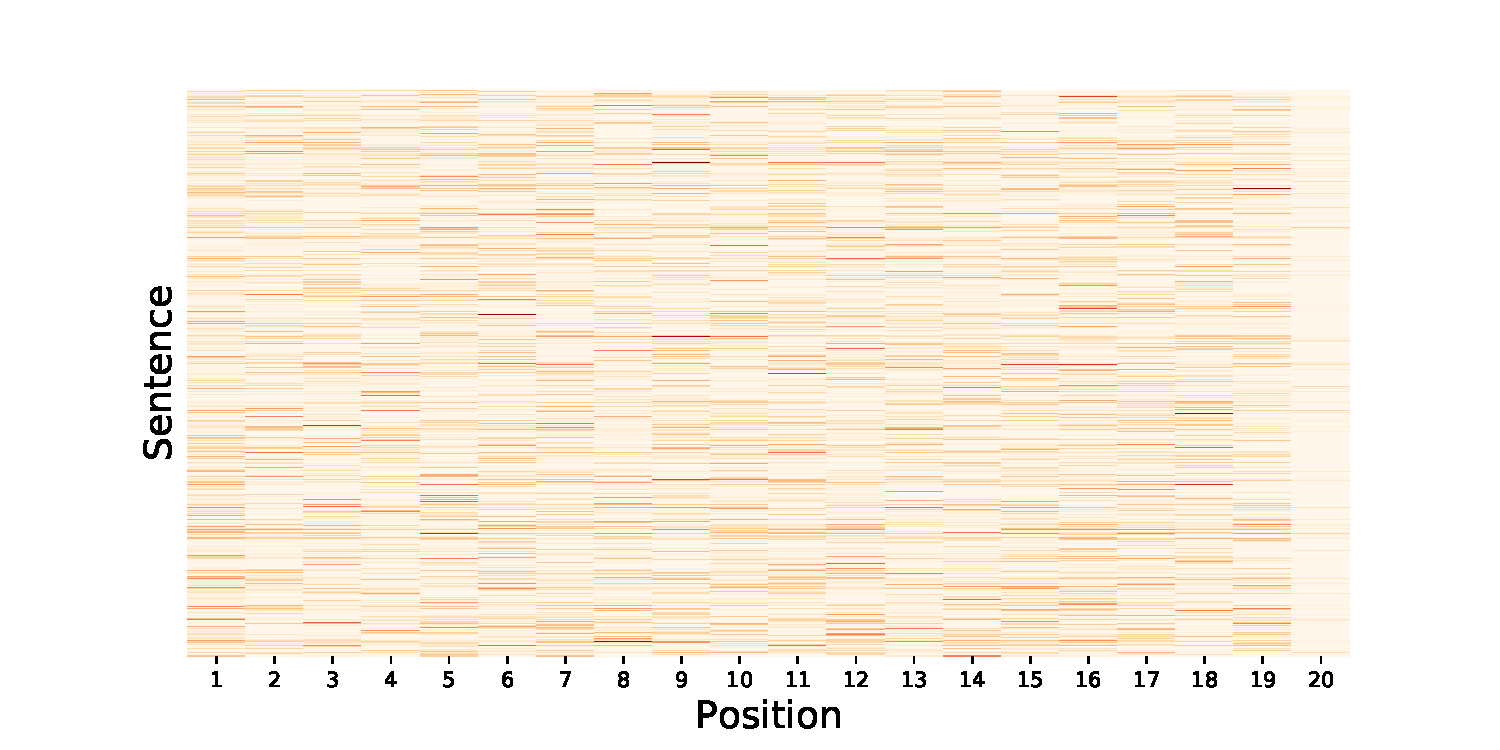
\includegraphics[width=\textwidth]{05-research-03/figs/lossesotro}
\caption{Prediction losses of 1000 randomly sampled sentences of the same length (20 tokens) from the training data. Darker means the model has less confidence predicting the word. \label{losepos}}
\end{center}
\end{figure}
The prediction loss of the token $i$ in the target sentence is conditioned on the source sentence and the target tokens generated up to the token in position $i$.
As a result, words that occur later in the sentence have more contextual evidence than words appearing earlier and this could lead to better prediction. 
We examine whether the position of the token in the sentence is a notable factor in prediction loss values.

We randomly sample 1000 sentences of the same length (20 tokens) from the training data and observe the confidence of the model in the prediction. 
Figure~\ref{losepos} shows the spread of prediction loss values in each position in the sentence. 
The only distinct pattern we observe is that the last position has consistently low prediction loss.
This is expected since the end-of-sentence symbol always follows the end of sentence markers, such as `.', `!', or `?'.
We observe that the average loss values are slightly higher for the first position ($12\%$ higher). 
However, other positions have very similar average losses.  
We conclude that the position in the sentence is not a significant factor in individual prediction losses.


\section{Conclusion} \label{btconc}

Motivated by our observations in Chapter~\ref{chapter:research-02} that synthesizing new context is useful for translation of rare words, we further explored in this chapter the impact of additional contexts on the translation of words that are difficult to predict by the baseline model. 
We asked:
 
\begin{enumerate}[label=\textbf{RQ2.\arabic* },wide = 0pt, leftmargin=2em]
\setlength\itemsep{1em}
 \setcounter{enumi}{2}
\item \acl{rq:bt1}

\medskip

\noindent In this chapter, we explored different aspects of the back-translation method to gain a better understanding of its performance.
Our analyses showed that the quality of the synthetic data has a small impact on the effectiveness of back-translation once there is sufficient training data available.
However, the ratio of synthetic to real training data plays a more critical role.
When the ratio of synthetic to real data is high, the model becomes biased towards noise in the synthetic data and the quality decreases.

Next, we examined the NMT model and found that words with high prediction losses after training benefit the most from additional back-translated data.
%We observed that words with high prediction losses in the original model undergo the most changes after training with synthetic data. 
While individual prediction losses are not a distinctive factor in identifying difficult words and same words in very similar contexts have high variance of prediction loss, by averaging these values we can successfully spot difficult words.
Our findings showed that, when original model has a low confidence in predicting words, the addition of contexts for those words to the training data increases the overall accuracy of the model on the unseen test set. %conc

\noindent 
Equipped with this information, we asked:

\item \acl{rq:bt2}

\medskip

\noindent As an alternative to random sampling target sentences for back-translation, we proposed targeted sampling and specifically targeted words that are difficult to predict.
%We proposed several variants of using the prediction loss in identifying relevant sentences to back-translate.
%We also used the contexts of difficult words as a feature to sample sentences for back-translation.
We found that data augmentation with the goal of increasing contexts for difficult-to-predict words improved the translation quality in German$\leftrightarrow$English. % by up to 1.7 {BLEU} points.
Interestingly, the proposed frequency-based sampling approach is a simple, yet effective strategy that is hard to outperform.
This indicates that signals from the data distribution are on par with signals from the failures of the model.

\end{enumerate}

 \noindent  This allows us to answer our more general question: 

\paragraph{Research Question 2:} \acl{rq:tdabt} 

\medskip

 \noindent In this chapter, we continued our study on the influence of having diverse contexts on translation quality. 
 We found that translation quality improves when we diversify the context of difficult words.
%In particular, we focused on the back-translation method and the distinct synthetic contexts that are generated with a reverse NMT model. 
%Despite the fact that back-translation has become a standard method in current NMT models, there is little research on understanding how models benefit from synthetic data.  
We investigated the effective method of back-translation for NMT and explored alternatives to the typically used random selection of target sentences that are to be back-translated into the source language.

\medskip

 \noindent  In Chapters~\ref{chapter:research-02} and~\ref{chapter:research-03}, we studied the impact of the availability of data and why models suffer from {a lack of} diverse contexts during training.
We proposed two main data augmentation approaches with multiple variants targeting different problems in translation.  
Both approaches proposed in Chapters~\ref{chapter:research-02} and~\ref{chapter:research-03} lead to improvements in translation quality.



